\documentclass[sigconf]{acmart}

\usepackage{booktabs} % For formal tables
\usepackage{listings}
\usepackage{amsmath} % AMS Math Package
\usepackage{amsthm} % Theorem Formatting
\usepackage{amssymb}	% Math symbols such as \mathbb
\usepackage{tikz}
\usepackage{siunitx}
\usepackage{graphicx}
\usepackage{minted} % code
\usetikzlibrary {positioning}

\newcommand{\curl}[1]{{\nabla} \times #1} % for curl

% Copyright
\setcopyright{none}

% DOI
\acmDOI{}

% ISBN
\acmISBN{}

%Conference
\acmConference{}{}{}

%\acmBooktitle{}
%\settopmatter{printacmref=false}

\begin{document}

\title{Simulating Turbulence with Recurrent Neural Networks }
\subtitle{}

\author{Robert Jendersie}

\maketitle

\section{Introduction}
In fluid dynamics, turbulence remains an unsolved problem. While the dynamics are described by the Navier-Stokes equations, a numerical simulation of sufficiently high resolution, where turbulence operates, remains infeasible. On a statistical level however, the different scales of frequencies are known to follow the Kolmogorov cascade, an observation which has been used to generate turbulence with plausible energy distributions and temporal coherence \cite{kim2008wavelet}. \\
Neural networks have enjoyed success in an increasingly wide range of problems, including classification, long term decision-making and image synthesis.
Recently, recurrent neural networks(RNNs) have been considered to predict chaotic physical systems; see \cite{vlachas2019forecasting} for a comparison off different approaches.
The possibility of having a RNN learn to simulate a turbulent flow is explored in this report.
\section{Network Architecture}
\begin{figure}
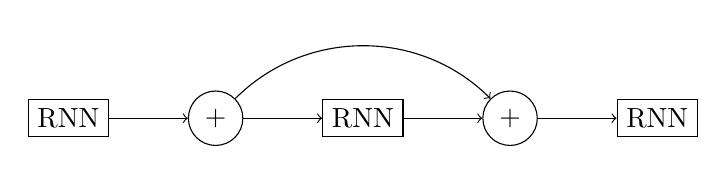
\begin{tikzpicture}
[add/.style={circle,draw},layer/.style={rectangle,draw}]
\node[layer] (rnn0) {RNN};
\node[add] (add0) [right=of rnn0] {+};
\node[layer] (rnn1) [right=of add0] {RNN};
\node[add] (add1) [right=of rnn1] {+};
\node[layer] (rnn2) [right=of add1] {RNN};
\draw [->] (rnn0.east) -- (add0.west);
\draw [->] (add0.east) -- (rnn1.west);
\draw [->] (add0) to [bend left=45] (add1);
\draw [->] (rnn1.east) -- (add1.west);
\draw [->] (add1.east) -- (rnn2.west);
\end{tikzpicture}
\caption{Residual Layers.}
\label{residualLayers}
\end{figure}
The objective of the network is to simulate the high resolution vector-field $\vec{u}$ for an arbitrary number of steps in a scene where turbulence occurs.
Instead of directly operating on $\vec{u}$, its vorticity $\zeta$
\[
\zeta = \curl{\vec{u}},
\]
is used. Assuming that $\vec{u}$ is divergence free, $\zeta$ is sufficient to reconstruct the vector-field. In 2D, the vorticity is a scalar-field, thus reducing the number of dimensions and making it easy to visualize.
\subsection{Inputs and Outputs}
As input, the full $\zeta$ from the previous time step and the current state of a lower resolution simulation are considered. 
In addition, parameters describing the variable parts of the scene, such as the size of the obstacle and inflow velocity may be given.
As output, the high resolution $\zeta$ is expected.
When operating on the spatial data, a stack of convolutional layers is used to extract important features and deconvolutional layers to create the full size output. Alternately, inputs and outputs can also be directly given in a frequency domain, in which case multiple dense layers with non-linear activation functions are applied to match the correct sizes.
\subsection{Recurrent Layers}
The main work is done by the recurrent layers, for which both Long Short-Term Memory(LSTM) and Gated Recurrent Units(GRU) are suitable. Where dimensions are compatible, residual connections are inserted, adding together the inputs and outputs of the current layer as shown by Figure~\ref{residualLayers}. This generally improves the training success, especially for longer networks, at small cost for both training and execution since no extra weights are needed and addition operations are cheap \cite{he2016deep}. \\
An important parameter of the units is their state-fullness. Usually RNNs are feed a fixed number of steps to predict the next step, after which the internal memory of each unit is reset to $0$. For a simulation, processing just one time step should yield the next one. Also, the training can impose some practical limits on the number of time steps given as input, which may be shorter than some long term dependencies. Thus, only state-full networks are considered.
%todo refs
\subsection{Frequency Domain}
\begin{itemize}
	\item frequency vs spatial
	\item conv, deconv, dense
\end{itemize}
\subsection{Common Options}
\begin{itemize}
	\item LSTM / GRU
	\item residual connections \cite{he2016deep}
	\item batch normalization
\end{itemize}
%%%%%%%%%%%%%%%%%%%%%%%%%%%%%%%%%%%%%%%%%%%%%%%%%%%%%%%%%%%%%%%%%%%%%%%%%%%%%%%
\section{Training Setup}
\begin{figure}
	\begin{tikzpicture}
	\node[anchor=south west,inner sep=0] (image) at (0,0) {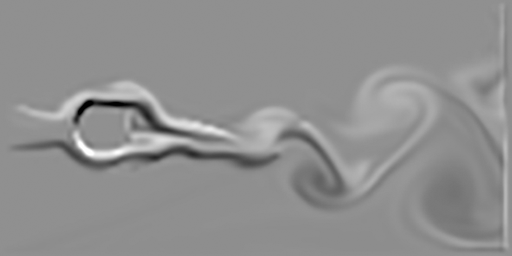
\includegraphics[width=0.45\textwidth]{imgs/scene.png}};
	\begin{scope}[x={(image.south east)},y={(image.north west)}]
		\draw[blue,ultra thick] (0.0,0.419) rectangle (0.05,0.581) node[above] {source};
		\draw[blue,ultra thick] (0.2,0.5) ellipse [x radius=0.05, y radius=0.1] (0.2,0.6) node[above] {obstacle};
	\end{scope}
	\end{tikzpicture}
	\caption{The Scene.}
	\label{trainingScene}
\end{figure}
The training setup, as shown rotated by $\ang{90}$ in Figure~\ref{trainingScene} consists of a source at the bottom, where smoke flows in and a circular obstacle above it. Through buoyancy, the smoke flows around the obstacle on both sides, causing turbulence in the area above. To add some variation, noise is applied to the inflow. Also the obstacle size can be changed and some random initial velocity is applied to the input.
%todo check this
Advection is computed with a second order semi Lagrange \\
Instead of a fixed size data set, the generator pattern is used. The numerical simulation can provide a continuous stream of new data, minimizing the risk of over-fitting. Also, usual processing such as shuffling and batching the data after each epoch pose problems with the consistent state of the network over multiple training steps.
\subsection{Stateful Recurrent Neural Networks}
As mentioned before, RNN layers use a special training process displayed in Figure~\ref{rnnTraining}. Instead of passing through one sample and back propagating the error, $k$ time steps are processed by a loop and only the final output is used in the error computation. During back propagation, the loop is unrolled, effectively stacking the same layer multiple times. 
\begin{figure}
	\begin{tikzpicture}
	[gap/.style={},layer/.style={rectangle,draw}]
	\node[gap]   (inp0) {$t_0$};
	\node[gap]   (inp1) [right=of inp0] {$t_1$};
	\node[layer] (rnn0) [below=of inp0] {LSTM};
	\node[layer] (rnn1) [right=of rnn0, below=of inp1] {LSTM};
	\node[gap]   (rnn2) [right=of rnn1] {$\dots$};
	\node[layer] (rnn3) [right=of rnn2] {LSTM};
	\node[gap]   (inp2) [right=of inp1, above=of rnn3] {$t_{k-1}$};
	\node[gap]   (outp) [below=of rnn3] {$t_k$};
	\draw [->] (inp0.south) -- (rnn0.north);
	\draw [->] (inp1.south) -- (rnn1.north);
	\draw [->] (inp2.south) -- (rnn3.north);
	\draw [->] (rnn0.east) -- (rnn1.west);
	\draw [->] (rnn1.east) -- (rnn2.west);
	\draw [->] (rnn2.east) -- (rnn3.west);
	\draw [->] (rnn3.south) -- (outp.north);
	\end{tikzpicture}
	\caption{A single LSTM layer in training.}
	\label{rnnTraining}
\end{figure}
While a larger window size $k$ may allow the network to pick up long term dependencies, the increased training time sets practical bounds and the impact of different choices is tested.\\
Processing multiple samples together as a batch and updating weights from the accumulated error is important both to speed up the training and to prevent over-fitting. However, for state-full networks, continuity across batches is required. Thus, batches of size $b$ would need to be build from $b$ different time-series. Instead of running multiple simulations a ring buffer of previous steps is kept. By choosing a sufficient distance $d$, a history of size $b \cdot d$ can be used to create batches of seemingly independent simulations. Let $p$ be the pointer to the current position of the ring buffer. Then after just one simulation step the next batch is constructed from the elements with indices
\[
ind_i = (p + i \cdot d) \mod (b \cdot d),
\]
where $i=0,\dots,b-1$.
Since tensorflow requires for state-full RNNs that the batch size is a fixed parameter, the trained model is impractical for the actual use case where just one time series should be simulated. Fortunately this issue, as well as the awkwardness of having to input multiple time steps to receive just one output, can be circumvented by building another model with the same architecture but $b=k=1$. Then the training results from \textit{modelT} can be transferred to \textit{modelP} via 
\begin{minted}{python}
modelP.set_weights(modelT.get_weights())
\end{minted}
\section{Evaluation}
\section{Conclusion}
\subsection{Limitations}
\subsection{Future Work}

\bibliographystyle{ieeetr}
%\bibliographystyle{ACM-Reference-Format}
%\nocite{*}
\bibliography{references}
\end{document}
